% Caratula y formato
\documentclass[12pt]{article}
\usepackage[utf8]{inputenc}
\usepackage[spanish]{babel}
\usepackage{a4wide}
\usepackage{caratula}
\usepackage{amsfonts}
\usepackage{placeins}

%%%%%%%%%%%%%%%%%%%%%%%%%%%%%
% Matrices 
\usepackage{amsmath}
\usepackage{mathtools}

\makeatletter
\renewcommand*\env@matrix[1][*\c@MaxMatrixCols c]{%
  \hskip -\arraycolsep
  \let\@ifnextchar\new@ifnextchar
  \array{#1}}
\makeatother

%%%%%%%%%%%%%%%%%%%%%%%%%%%%
% Pseudocódigo
\usepackage[noend]{algpseudocode}
\usepackage{algorithm}
\algnewcommand{\IfThenElse}[3]{\State \algorithmicif\ #1\ \algorithmicthen\ #2\ \algorithmicelse\ #3}
\algnewcommand{\IfThen}[2]{\State \algorithmicif\ #1\ \algorithmicthen\ #2}

% Comandos para tener Input y Output en el enviroment de algorithmic
%\floatname{algorithm}{Procedure}
\renewcommand{\algorithmicrequire}{\textbf{Input:}}
\renewcommand{\algorithmicensure}{\textbf{Output:}}

% Funciones de algorithmic sin nombre en mayuscula
% https://tex.stackexchange.com/questions/150184/how-to-avoid-uppercase-function-name-while-using-function
\algrenewcommand\textproc{} % Used to be \textsc

%%%%%%%%%%%%%%%%%%%%%%%%%%%%

\usepackage{hyperref}

% Comandos redefinidos
% https://tex.stackexchange.com/questions/69358/how-to-style-equation-label-and-reference-differently
\makeatletter
\def\tagform@#1{\maketag@@@{(\ignorespaces{#1}\unskip\@@italiccorr)}}
\renewcommand{\eqref}[1]{\textbf{eq. (\ref{#1})}}

% Distinto de \algref de algorithmicx
% Con esto podemos referenciar todo un algoritmo (quizas es mejor meterlo en una figura)
\newcommand{\algoref}[1]{\textbf{alg. (\ref{#1})}}
\makeatother

%%%%%%%%%%%%%%%%%%%%%%%%%%%%

\usepackage[shortlabels]{enumitem}

%%%%%%%%%%%%%%%%%%%%%%%%%%%%
% Figuras
\usepackage{svg}
\usepackage{caption}
\usepackage{subcaption}
\newcommand{\figref}[1]{\textbf{fig.} \ref{#1}}

%%%%%%%%%%%%%%%%%%%%%%%%%%%%

\materia{Métodos numéricos}
\submateria{2do cuatrimestre 2023}
\titulo{Trabajo práctico 1}
\subtitulo{Eliminación gaussiana, matrices tridiagonales y difusión}
\integrante{Tomás Bossi}{50/17}{tomasbossi97@gmail.com}
\integrante{Ignacio Enrique Niesz}{722/10}{ignacio.niesz@gmail.com}
\integrante{Brian Ivan Rios}{917/19}{ivan.rios2010@gmail.com}

\setlength{\parindent}{0cm}
\setlength{\parskip}{2mm}

\begin{document}

\maketitle
\tableofcontents 

\clearpage
\section{Introducción}

Cualquier sistema de ecuaciones lineales puede ser representado en forma matricial como $Ax=b$, donde $A$ es la matriz de los coeficientes que acompañan a cada una de las incognitas, $x$ es el vector de incognitas y $b$ es el vector de términos independientes. Resolver un sistema de ecuaciones lineales significa, entonces, dados $A$ y $b$ encontrar $x$ tal que $Ax=b$. Son particularmente interesantes los sistemas con igual cantidad de ecuaciones que incognitas, representables por una matriz de coeficientes $A$ cuadrada, que pueden según $A$ y $b$ no tener solución, tener solución única, o tener infinitas soluciones.

Existen algoritmos que permiten hallar la solución única de un dado sistema de ecuaciones, si es que tal solución existe. Los más conocidos y sencillos de estos algoritmos son los de eliminación gaussiana (EG), que en sus versiones más básicas consisten en realizar operaciones elementales entre filas que convierten al sistema en sistemas equivalentes (con el mismo vector solución $x$) progresivamente simplificados. Una vez que se llega a un sistema equivalente suficientemente sencillo, que en general consiste en un sistema en el que la matriz de coeficientes es triangular superior, los elementos de $x$ son despejados uno por uno. Todos los algoritmos de EG se basan en la operación elemental de reemplazo de una fila por la resta entre sí misma y un múltiplo de otra. Algunos algoritmos usan además la operación elemental de intercambio entre filas para resolver sistemas de otra manera irresolubles y disminuir el error numérico en las soluciones halladas, a lo que se le denomina ''pivoteo parcial''\cite{burden}\cite{metnum_EG}.

Los algoritmos de EG de propósito general, diseñados para sistemas dados por cualquier matriz de coeficientes cuadrada, son de complejidad $O(n^3)$. Para matrices ralas (con la mayoría de sus elementos nulos) pertenecientes a una dada familia puede ser posible diseñar algoritmos de una complejidad menor. Un caso trivial es el de los sistemas diagonales de solución única (con matriz diagonal, sin ceros en la diagonal), que ya están prácticamente resueltos. Estos sistemas requieren de a lo sumo $n$ divisiones para hallar $x$, y son por lo tanto de complejidad $O(n)$. Para sistemas tridiagonales (con matriz de coeficientes tridiagonal), se sabe que puede diseñarse un algoritmo que también es de complejidad $O(n)$.

El desarrollo de este trabajo puede ser dividido en cuatro partes. En la primera (sección \ref{sistemas_de_ecuaciones}) se diseñaron algoritmos de EG de propósito general sin y con pivoteo parcial (\ref{sistemas_de_ecuaciones_EG_sin} y \ref{sistemas_de_ecuaciones_EG_con}) y se analizaron casos particulares de uso interesantes (\ref{sistemas_de_ecuaciones_casos}). En la segunda parte (sección \ref{EG_tridiagonales}) se desarrolló un algoritmo de complejidad $O(n)$ específico a sistemas tridiagonales (\ref{EG_tridiagonales_sin_precomputo}), y se lo mejoró separándolo en una primera etapa de precómputo y una segunda etapa de resolución de el o los sistemas lineales dados (\ref{EG_tridiagonales_con_precomputo}). En la tercera parte (sección \ref{tiempos}) se realizaron análisis de los tiempos de cómputo de los algoritmos diseñados, estudiando entre otras cosas su dependencia con el tamaño de las matrices input y verificando que sus complejidades algorítmicas sean las esperadas. Finalmente, la cuarta parte del desarrollo (sección \ref{aplicaciones}) explora aplicaciones de los sistemas tridiagonales, en particular a los problemas de la búsqueda de funciones a partir de sus derivadas segundas (\ref{aplicaciones_laplaciano}) y al de la difusión en el tiempo y el espacio en una dimensión (\ref{aplicaciones_difusion}).

\clearpage
\section{Sistemas de ecuaciones}
\label{sistemas_de_ecuaciones}

\subsection{Eliminación gaussiana sin pivoteo}
\label{sistemas_de_ecuaciones_EG_sin}

El algoritmo de EG sin pivoteo (\algoref{alg:eg_sin_pivoteo}) es el más sencillo y elemental de los algoritmos de su tipo, y consta de dos etapas. La primera consiste en eliminar los elementos debajo de la diagonal de la matriz aumentada de coeficientes, yendo desde la primera fila hasta la última y usando como pivote al elemento en la diagonal correspondiente a cada paso de la triangulación (\algoref{alg:triangulación_sin_pivoteo}). Si el algoritmo encuentra un 0 en la posición de la diagonal que corresponde al paso actual de triangulación, no puede continuar ni hallar la solución del sistema. Si el algoritmo termina de triangular a la matriz y no quedan elementos nulos en su diagonal puede realizarse la segunda etapa, que consiste en despejar el valor de todos los elementos del vector solución $x$, yendo desde la última fila de la matriz hacia la primera, a lo que se le conoce como \textit{backwards substitution} (\algoref{alg:solución_única}).

\begin{algorithm}[H]
\begin{algorithmic}[1]
\Require{$A$ matriz de coeficientes cuadrada}
\Require{$b$ vector de términos independientes del sistema Ax=b}
\Ensure{$x$ vector columna solución única del sistema Ax=b. Si no existe solución única o no puede encontrarse sin realizar pivoteo, devuelve una excepción}
\Function{$solucion\_sistema\_lineal\_eliminacion\_gaussiana\_sin\_pivoteo$}{$A$, $b$}
    \State $A' \gets concatenar(A, b)$ \Comment{$A'$ es la matriz aumentada}
    \State $A' \gets escalonar\_matriz\_sin\_pivoteo(A')$ \Comment{\algoref{alg:triangulación_sin_pivoteo}}
    \State $x \gets solucion\_unica\_sistema\_lineal(A', 0)$ \Comment{\algoref{alg:solución_única}}
    \State \textbf{return} $x$
\EndFunction
\end{algorithmic}
\caption{EG sin pivoteo}
\label{alg:eg_sin_pivoteo}
\end{algorithm}

\begin{algorithm}[H]
\begin{algorithmic}[1]
\Require{$A'$ matriz de coeficientes aumentada de dimensiones $n$\texttt{x}$n+1$}
\Ensure{$A'$ matriz de coeficientes aumentada triangulada sin pivoteo. Si no puede realizarse la triangulación sin pivoteo (se encuentra un 0 en la diagonal en algún paso) devuelve una excepción}
\Function{$escalonar\_matriz\_sin\_pivoteo$}{$A'$}
    \For{$i = 1 \hdots n$}
        \If{$a'_{ii}== 0$ \&\& $a'_{i+1,...,n;i} == 0$}
            \State \textbf{then return Exception:} ''No puede encontrarse solución única''
        \EndIf
        \For{$j = i+1 \hdots n$}
            % \If{$a'_{ji} \neq 0$}
            \State $m_{ij} \gets a'_{ji}/a'_{ii}$
            \State $A'_j \gets A'_j - A'_i * m_{ij}$ \Comment{\algoref{alg:suma_matricial} y \algoref{alg:producto_por_escalar}}
            % \EndIf
        \EndFor
    \EndFor
    \State \textbf{return} $A'$
\EndFunction
\end{algorithmic}
\caption{Triangulación sin pivoteo}
\label{alg:triangulación_sin_pivoteo}
\end{algorithm}

\begin{algorithm}[H]
\begin{algorithmic}[1]
\Require{$A'$ matriz de coeficientes aumentada triangulada de dimensiones $n$\texttt{x}$n+1$}
\Require{$atol$ tolerancia absoluta para la comparación con el 0}
\Ensure{$x$ vector columna solución única del sistema Ax=b. Si no existe solución única o no puede encontrarse sin realizar pivoteo, devuelve una excepción Si en algún paso se debe dividir por un número cercano a 0 (cercano de acuerdo a $atol$), imprime una advertencia}
\Function{$solucion\_unica\_sistema\_lineal$}{$A'$}
    \State $x \gets [\phantom{.}]$
    \For{$i = n \hdots 1$}
        \State \textbf{if} $a'_{ii}== 0$ \textbf{then return Exception:} ''No puede encontrarse solución única''
        \State \textbf{if} $|a'_{ii}| < atol$ \textbf{then print:} ''Advertencia: división por valor cercano a 0''
        \State $b_i \gets a'_{i(n+1)}$ \Comment{término independiente}
        \State $suma\_terminos \gets x \cdot \begin{bsmallmatrix}a'_{i(i+1)} & a'_{i(i+2)} & \hdots & a'_{in}\end{bsmallmatrix}$ \Comment{\algoref{alg:producto_escalar}}
        \State $x_i \gets (b_{i} - suma\_terminos)/a_{ii}$
        \State $x \gets concatenar([x_i], x)$ \Comment{agrega $x_i$ al principio de $x$}
    \EndFor
    \State \textbf{return} $x$
\EndFunction
\end{algorithmic}
\caption{Solución única de sistema pretriangulado}
\label{alg:solución_única}
\end{algorithm}

\subsection{Eliminación gaussiana con pivoteo}
\label{sistemas_de_ecuaciones_EG_con}

El algoritmo sin pivoteo puede ser levemente modificado para incorporar pivoteo parcial, que implica la posibilidad de realizar intercambios entre filas de la matriz aumentada de coeficientes (\algoref{alg:eg_con_pivoteo}, \algoref{alg:triangulación_con_pivoteo}). Como se ejemplificará en la sección \ref{sistemas_de_ecuaciones_casos}, esto permite resolver sistemas que son irresolubles sin pivoteo. Para intercambiar filas el algoritmo busca el mejor pivote posible, aquel elemento de la columna a ser eliminada (sobre la diagonal de la matriz o debajo de ella) de valor máximo en módulo. Esto evita divisiones por números pequeños, reduciendo el error numérico en las soluciones halladas.

% El algoritmo sin pivoteo puede ser levemente modificado para incorporar pivoteo parcial, que implica la posibilidad de realizar intercambios entre filas de la matriz aumentada de coeficientes (\algoref{alg:triangulación_con_pivoteo}). Como se ejemplificará en la sección \ref{sistemas_de_ecuaciones_casos}, esto permite resolver sistemas que son irresolubles sin pivoteo. Para intercambiar filas el algoritmo busca el mejor pivote posible, aquel elemento de la columna a ser eliminada (sobre la diagonal de la matriz o debajo de ella) de valor máximo en módulo. Esto evita divisiones por números pequeños, reduciendo el error numérico en las soluciones halladas.

\begin{algorithm}[H]
\begin{algorithmic}[1]
\Require{$A$ matriz de coeficientes cuadrada}
\Require{$b$ vector de términos independientes del sistema Ax=b}
\Require{$atol$ tolerancia absoluta para la comparación con el 0}
\Ensure{$x$ vector columna solución única del sistema Ax=b. Si no existe solución única, devuelve una excepción}
\Function{$solucion\_sistema\_lineal\_eliminacion\_gaussiana\_pivoteo\_parcial$}{$A$, $b$, $atol$}
    \State $A' \gets concatenar(A, b)$ \Comment{$A'$ es la matriz aumentada}
    \State $A' \gets escalonar\_matriz\_pivoteo\_parcial(A', atol)$ \Comment{\algoref{alg:triangulación_con_pivoteo}}
    \State $x \gets solucion\_unica\_sistema\_lineal(A', atol)$ \Comment{\algoref{alg:solución_única}}
    \State \textbf{return} $x$
\EndFunction
\end{algorithmic}
\caption{EG con pivoteo parcial}
\label{alg:eg_con_pivoteo}
\end{algorithm}

\begin{algorithm}[H]
\begin{algorithmic}[1]
\Require{$A'$ matriz de coeficientes aumentada de dimensiones $n$\texttt{x}$n+1$}
\Require{$atol$ tolerancia absoluta para la comparación con el 0}
\Ensure{$A'$ matriz de coeficientes aumentada triangulada con pivoteo parcial. Si se determina que no existe solución única para el sistema $Ax=b$ (se encuentra que 0 es el mejor pivote en algún paso) devuelve una excepción}
\Function{$escalonar\_matriz\_pivoteo\_parcial$}{$A'$, $atol$}
    \For{$i = 0 \hdots n$}
        \State $p \gets a'_{ii}$
        \State $idp \gets i$
        \For{$j = i+1 \hdots n$}
            \If{$|a'_{ji}| > |p|$}
                \State $p \gets a'_{ji}$
                \State $idp \gets j$
            \EndIf
        \EndFor
        \State $fila\_pivote \gets A'_{idp}$
        \State $A'_{idp} \gets A'_i$
        \State $A'_i \gets fila\_pivote$
        \State \textbf{if} $p== 0$ \textbf{then return Exception:} ''No puede encontrarse solución única''
        \State \textbf{if} $|p| < atol$ \textbf{then print:} ''Advertencia: división por valor cercano a 0''
        \For{$j = i+1 \hdots n$}
            % \If{$a'_{ji} \neq 0$}
            \State $m_{ij} \gets a'_{ji}/p$
            \State $A'_j \gets A'_j - A'_i * m_{ij}$ \Comment{\algoref{alg:suma_matricial} y \algoref{alg:producto_por_escalar}}
            % \EndIf
        \EndFor
    \EndFor
    \State \textbf{return} $A'$
\EndFunction
\end{algorithmic}
\caption{Triangulación con pivoteo parcial}
\label{alg:triangulación_con_pivoteo}
\end{algorithm}

\subsection{Observaciones sobre sistemas particulares} 
\label{sistemas_de_ecuaciones_casos}

Sean los siguientes sistemas de ecuaciones:
\[
(a) 
\begin{bmatrix}
    0  &  1      \\
    1  &  2      
\end{bmatrix}
\begin{bmatrix}
    x_1          \\
    x_2      
\end{bmatrix} 
= 
\begin{bmatrix}
    1            \\
    1 
\end{bmatrix} 
% \phantom{........}
\phantom{..}
(b) 
\begin{bmatrix}
    1  &  1      \\
    1  &  1      
\end{bmatrix}
\begin{bmatrix}
    x_1          \\
    x_2      
\end{bmatrix} 
= 
\begin{bmatrix}
    1            \\
    1 
\end{bmatrix}
% \phantom{........}
\phantom{..}
(c) 
\begin{bmatrix}
    2\epsilon & 2 \\
    \epsilon & 2-\epsilon
\end{bmatrix}
\begin{bmatrix}
    x_1          \\
    x_2          \\
    % x_3          \\
    % x_4          \\
    % x_5          \\
\end{bmatrix} 
= 
\begin{bmatrix}
    2+\beta      \\
    2            \\
    % 17           \\
    % 7            \\
    % 17           \\
\end{bmatrix} 
\]

Donde $\epsilon = 10^{-15}$ y $\beta = 2.220446049250313\times 10^{-15}$. $(a)$ Es un sistema no resoluble realizando EG sin pivoteo (\algoref{alg:eg_sin_pivoteo}) pero sí con pivoteo parcial (\algoref{alg:eg_con_pivoteo}), $(b)$ es un sistema no resoluble por EG con o sin pivoteo parcial por tener infinitas soluciones, y $(c)$ es un sistema cuya solución exacta es aproximadamente $x_{real} = \begin{bsmallmatrix}1 & 1\end{bsmallmatrix}^T$, pero que al aplicarle EG con pivoteo parcial con $atol = 10\epsilon$ (\algoref{alg:eg_con_pivoteo}) ocasiona que dispare la advertencia por división por un número pequeño y produce una solución incorrecta a causa de error numérico, aproximadamente $x_{exp} = \begin{bsmallmatrix}1.11 & 1\end{bsmallmatrix}^T$. La matriz del sistema $(c)$ tiene número de condición de aproximadamente $\kappa = 4\times10^{15}$.

% \begin{enumerate}[label=(\alph*)]
%     \item Es un sistema no resoluble realizando EG sin pivoteo (\algoref{alg:eg_sin_pivoteo}) pero sí con pivoteo parcial (\algoref{alg:eg_con_pivoteo}).
%     \item Es un sistema no resoluble por EG, con o sin pivoteo parcial, por tener infinitas soluciones.
%     \item Es un sistema cuya solución exacta es $x_{real} = \begin{bsmallmatrix}-1\\1\end{bsmallmatrix}$, pero que al aplicarle EG con pivoteo parcial con $atol = 0.01$ (\algoref{alg:eg_con_pivoteo}) ocasiona que dispare la advertencia por división por un número pequeño y produce una solución aproximada por error numérico ($x_{exp} = \begin{bsmallmatrix}-0.9999999999999551\\0.9999999999999776\end{bsmallmatrix}$).
% \end{enumerate}

\clearpage
\section{Sistemas de ecuaciones tridiagonales}
\label{EG_tridiagonales}

La representación matricial de un sistema de ecuaciones tridiagonal es de la forma:
 
\begin{equation}
\begin{bmatrix}
   b_1 & c_1 &        &        &  0      \\
   a_2 & b_2 & c_2    &        &         \\
       & a_3 & b_3    & \ddots &         \\
       &     & \ddots & \ddots & c_{n-1} \\
   0   &     &        & a_n    & b_n
\end{bmatrix}
\begin{bmatrix}
   x_1    \\
   x_2    \\
   x_3    \\
   \vdots \\
   x_n
\end{bmatrix}
=
\begin{bmatrix}
   d_1    \\
   d_2    \\
   d_3    \\
   \vdots \\
   d_n
\end{bmatrix}
.
\label{eq:DEF_TRIDIAGONAL}
\end{equation}

La solución del sistema queda determinada por 4 vectores:  $a$, $b$, $c$ (las diagonales) y $d$ (el vector de términos independientes), todos de largo $n$, d\'onde se asume que $a_{1} = c_{n} = 0$. Esto permite diseñar un algoritmo más eficiente en tiempo y espacio que el de EG convencional.

\subsection{Eliminaci\'on gaussiana para sistemas tridiagonales}
\label{EG_tridiagonales_sin_precomputo}

La estructura de los sistemas tridiagonales permite el desarrollo de un algoritmo que reduce la complejidad de resoluci\'on del sistema de $O(n^{3})$ a $O(n)$, descripto en \algoref{alg:EG_tridiagonal_sin_precomputo}. 

\begin{algorithm}[H]
\begin{algorithmic}[1]
\Require{$a$, $b$, $c$, $d$ vectores de largo $n$ con $a_1 = c_n = 0$}
\Require{$atol$ tolerancia absoluta para la comparación con el 0}
\Ensure{$x$ vector columna solución única del sistema tridiagonal. Si no existe solución única, devuelve una excepción}
\Function{solucion\_sistema\_tridiagonal\_eliminacion\_gaussiana\_cuidadosa}{$a$, $b$, $c$, $d$, $atol$}
    \State $x \gets d$ \Comment{copia profunda}
    \For{$i = 1 \hdots n-1$}
         \State \textbf{if} $b_i==0$ \textbf{then return Exception:} ''No puede encontrarse solución única''
        \State \textbf{if} $|b_i| < atol$ \textbf{then print:} ''Advertencia: división por valor cercano a 0''
        \State $\alpha \gets a_{i+1}/b_i$
        \State $b_{i+1} \gets b_{i+1} - \alpha c_i$ 
        \State $d_{i+1} \gets d_{i+1} - \alpha d_{i}$
    \EndFor
    \State \textbf{if} $b_n==0$ \textbf{then return Exception:} ''No puede encontrarse solución única''
    \For{$i = n \hdots 2$}
        \State \textbf{if} $|b_i| < atol$ \textbf{then print:} ''Advertencia: división por valor cercano a 0''
        \State $\alpha \gets c_{i-1}/b_i$
        \State $d_{i-1} \gets d_{i-1} - \alpha d_{i}$
        \State $x_i \gets d_i/b_i$
    \EndFor
    \State $x_1 \gets d_1/b_1$
    \State \textbf{return} $x$
\EndFunction
\end{algorithmic}
\caption{Solución única de sistema tridiagonal}
\label{alg:EG_tridiagonal_sin_precomputo}
\end{algorithm}

En un primer paso, el algoritmo recorre a $b$ desde adelante hacia atrás para anular por completo al vector $a$. Esto genera cambios sobre $b$ y $d$, pero no sobre $c$. En un segundo paso, recorre al $b$ modificado desde atrás hacia adelante para anular c, modificando nuevamente a $d$. Esto resulta en un único vector $b'$ que es diagonal única de la representación matricial del sistema, y un $d'$ que es el vector de términos independientes modificado por todas las operaciones realizadas. A partir de $b'$ y $d'$, hallar $x$ (si existe) es trivial.

\subsection{Eliminaci\'on gaussiana en dos etapas para sistemas tridiagonales (precómputo)} \label{dos-etapas}
\label{EG_tridiagonales_con_precomputo}

Si se desea resolver una serie de sistemas de ecuaciones para una misma matriz de coeficientes, variando nada más que el vector de términos independientes, recomputar la enteritud de la EG para cada sistema es un desperdicio de recursos. Resulta más eficiente computar el resultado de realizar EG sobre la matriz de coeficientes una única vez, conservando de alguna manera toda la información necesaria sobre las operaciones realizadas en el proceso. Luego, esas mismas operaciones pueden ser aplicadas en el orden adecuado sobre cualquier vector de términos independientes sin necesidad de volver a operar sobre la matriz de coeficientes. En el caso de sistemas tridiagonales esto es particularmente sencillo, y el precómputo consiste en simplemente aplicar una versión modificada de \algoref{alg:EG_tridiagonal_sin_precomputo} que no recibe $d$ y devuelve $b'$ y el vector de las operaciones realizadas (los factores multiplicativos calculados) en orden. (\algoref{alg:EG_tridiagonal_precomputo}). Luego otro algoritmo puede ser utilizado para, a partir de $b'$, el vector de operaciones, y un vector $d$, operar sobre $d$ y resolver el sistema trivialmente (\algoref{alg:sol_tridiag_precomputo}).

\begin{algorithm}[H]
\begin{algorithmic}[1]
\Require{$b'$ vector diagonal del sistema diagonal}
\Require{$d$ vector de términos independientes del sistema tridiagonal original}
\Require{$operaciones$ vector de factores multiplicativos necesarios para operar sobre $d$}
\Require{$atol$ tolerancia absoluta para la comparación con el 0}
\Ensure{$x$ vector columna solución única del sistema tridiagonal original. Si no existe solución única, devuelve una excepción}
\Function{solucion\_sistema\_tridiagonal\_precomputado}{$b'$, $d$, $operaciones$, $atol$}
    \State $x \gets d$ \Comment{copia profunda}
    \State $d' \gets preoperar\_d\_sistema\_tridiagonal(d, operaciones)$ \Comment{\algoref{alg:preoperar_d}}
    \For{$i = 1 \hdots n$}
         \State \textbf{if} $b'_i==0$ \textbf{then return Exception:} ''No puede encontrarse solución única''
        \State \textbf{if} $|b'_i| < atol$ \textbf{then print:} ''Advertencia: división por valor cercano a 0''
        \State $x_i \gets d'_i/b'_i$
        \EndFor
    \State \textbf{return} $x$
\EndFunction
\end{algorithmic}
\caption{Solución única de sistema tridiagonal con precómputo}
\label{alg:sol_tridiag_precomputo}
\end{algorithm}

\begin{algorithm}[H]
\begin{algorithmic}[1]
\Require{$d$ vector de longitud $n$ de los términos independientes del sistema tridiagonal}
\Require{$operaciones$ vector de factores multiplicativos necesarios para operar sobre $d$, de longitud $2*(n - 1)$}
\Ensure{$d$ vector de términos independientes modificado de acuerdo a $operaciones$ para corresponder con su sistema diagonal asociado}
\Function{preoperar\_d\_sistema\_tridiagonal}{$d$, $operaciones$}
    \For{$i = 1 \hdots n-1$}
        \State $d_{i+1} \gets d_{i+1} - operaciones_i*d_i$ 
    \EndFor
    \For{$i = n \hdots 2$}
        \State $d_{i-1} \gets d_{i-1} - operaciones_{2n-i}*d_i$ 
    \EndFor
    \State \textbf{return} $d$
\EndFunction
\end{algorithmic}
\caption{Preoperaciones sobre el vector de términos independientes}
\label{alg:preoperar_d}
\end{algorithm}

\begin{algorithm}[H]
\begin{algorithmic}[1]
\Require{$a$, $b$, $c$ vectores de largo $n$ con $a_1 = c_n = 0$}
\Require{$atol$ tolerancia absoluta para la comparación con el 0}
\Ensure{$b'$ vector diagonal del sistema diagonal}
\Ensure{$operaciones$ vector de factores multiplitcativos utilizados en la EG, en orden}
\Function{precomputo\_sistema\_tridiagonal\_EG\_cuidadosa}{$a$, $b$, $c$, $atol$}
    \State $operaciones \gets [\phantom{.}]$
    \For{$i = 1 \hdots n-1$}
         \State \textbf{if} $b_i==0$ \textbf{then return Exception:} ''No puede encontrarse solución única''
        \State \textbf{if} $|b_i| < atol$ \textbf{then print:} ''Advertencia: división por valor cercano a 0''
        \State $\alpha \gets a_{i+1}/b_i$
        \State $operaciones \gets concatenar(operaciones, [\alpha])$ \Comment{agrega $\alpha$ al final de $operaciones$}
        \State $b_{i+1} \gets b_{i+1} - \alpha c_i$
    \EndFor
    \State \textbf{if} $b_n==0$ \textbf{then return Exception:} ''No puede encontrarse solución única''
    \For{$i = n \hdots 2$}
        \State \textbf{if} $|b_i| < atol$ \textbf{then print:} ''Advertencia: división por valor cercano a 0''
        \State $\alpha \gets c_{i-1}/b_i$
        \State $operaciones \gets concatenar(operaciones, [\alpha])$
    \EndFor
    \State \textbf{return} $b, operaciones$
\EndFunction
\end{algorithmic}
\caption{EG para sistemas tridiagonales (precómputo)}
\label{alg:EG_tridiagonal_precomputo}
\end{algorithm}

\clearpage
\section{Tiempos de ejecuci\'on}
\label{tiempos}

Para medir tiempos de cómputo en función del tamaño de la matriz input, se eligió como métrica al tiempo de ejecución mínimo a partir de $n\_rep$ repeticiones. Más especificamente, para cada algoritmo y bajo cada condición, se utilizó al comando \texttt{\%timeit} de IPython\cite{timeit} para realizar $n\_rep*k$ mediciones individuales totales, separadas en grupos de $k$ ejecuciones cada uno. En todos los casos se midió el \textit{CPU User time}\cite{patterson}. El tiempo informado $MT$ (por Mejor Tiempo) para un dado algoritmo para un dado tamaño del input es el mínimo de los tiempos promedio de cada uno de esos $n\_rep$ grupos de $k$ ejecuciones:

$$MT = \min\limits_{i = 1,...,n\_rep} {\{\frac{1}{k}\sum\limits_{j = 1}^{k}{med_{ij}}\}}$$

Donde $med_{ij}$ es la medición individual $j$ (de $k$ mediciones por grupo) del grupo de mediciones $i$ (de $n\_rep$ grupos).

Las matrices de prueba fueron en todos los casos precomputadas, de forma tal que el tiempo necesario para su generación no forma parte de las mediciones. Para la comparación entre tanto los algoritmos de EG común con y sin pivoteo como entre EG con pivoteo y EG para tridiagonales, se procuró para cada tamaño de matriz analizado siempre utilizar al mismo grupo de $n\_rep*k$ matrices precomputadas. En todos los casos se usó al vector columna $(1, 1, \hdots, 1)^T$ de la dimensión correspondiente como vector de términos independientes.

Para el caso particular de la medición de tiempos de cómputo para comparar al algoritmo de EG para tridiagonales con y sin precómputo, se utilizó como métrica al mínimo de los tiempos totales de ejecución de cada uno de los $n\_rep$ grupos, que equivale simplemente a calcular $k*MT$. Se utilizaron únicamente 4 matrices tridiagonales generadas al azar, una para cada tamaño de matriz analizado ($32$\texttt{x}$32$, $64$\texttt{x}$64$, $96$\texttt{x}$96$ y $128$\texttt{x}$128$).

Las mediciones se resumen en las figuras \ref{fig:EG_sin_vs_con_pivoteo}, \ref{fig:EG_tridiagonales} y \ref{fig:EG_tridiag_sin_vs_con_precomp}. En todos los casos, se obtuvieron los resultados esperados de acuerdo a nuestros conocimientos previos sobre los algoritmos analizados. 

Se encontró que los algoritmos de EG común con y sin pivoteo parcial son muy similares entre sí en cuanto a sus tiempos de cómputo, por lo menos para los tamaños de matriz analizados. Los resultados comprueban además que ambos algoritmos son aproximadamente $O(n^3)$ (figura \ref{fig:EG_sin_vs_con_pivoteo}).

Por otro lado, se observó que al operar sobre sistemas tridiagonales el algoritmo diseñado específicamente para este tipo de matrices es muy significativamente más rápido que el algoritmo de EG común con pivoteo parcial (figura \ref{fig:EG_con_pivoteo_vs_tridiagonales}). Por ejemplo, para el caso puntual de matrices tridiagonales de tamaño $128$\texttt{x}$128$, el algoritmo de EG para tridiagonales es más de 200 veces más rápido. Esta diferencia en velocidad se debe mayormente a la diferencia cualitativa en la complejidad de estos algoritmos, siendo el algorítmo de EG para tridiagonales de complejidad $O(n)$ (figura \ref{fig:EG_tridiagonales_solo}).

\clearpage
\begin{figure}[!ht]
    \centering\includesvg[width=0.6\textwidth]{imgs/EG_sin_vs_con_pivoteo.svg}
    \caption{Tiempos de cómputo vs tamaño de la matriz input para los algoritmos de EG convencional con y sin pivoteo (\algoref{alg:eg_con_pivoteo}, \algoref{alg:eg_sin_pivoteo}). Se utilizó $k=10$ y $n\_rep=100$, con 1000 matrices triangulares inferiores pregeneradas para cada tamaño. Se muestra también el mejor ajuste por cuadrados mínimos a los datos (sin pivoteo) con un polinomio grado 3.}
    \label{fig:EG_sin_vs_con_pivoteo}
\end{figure}

\begin{figure}[!ht]
    \centering
    \begin{subfigure}[b]{0.475\textwidth}
        \centering
        \includesvg[width=\textwidth]{imgs/EG_con_pivoteo_vs_tridiag_log.svg}
        \caption{}
        \label{fig:EG_con_pivoteo_vs_tridiagonales}
    \end{subfigure}
    \hfill
    \begin{subfigure}[b]{0.45\textwidth}
        \centering
        \includesvg[width=\textwidth]{imgs/EG_tridiag.svg}
        \caption{}
        \label{fig:EG_tridiagonales_solo}
    \end{subfigure}
    \caption{Tiempos de cómputo vs tamaño de la matriz input para los algoritmos de EG convencional con pivoteo y de EG para matrices tridiagonales sin precómputo (\algoref{alg:eg_con_pivoteo}, \algoref{alg:EG_tridiagonal_sin_precomputo}). \textbf{(a)} Comparación entre ambos algoritmos en escala logarítmica. Se utilizó $k=50$ y $n\_rep=100$, con 5000 matrices tridiagonales pregeneradas para cada tamaño. \textbf{(b)} Resultados para el algoritmo de EG para matrices tridiagonales sin precómputo con $k=1000$, $n\_rep=200$ y 200000 triplas de diagonales de matrices tridiagonales pregeneradas.}
    \label{fig:EG_tridiagonales}
\end{figure}

\begin{figure}[!ht]
    \centering\includesvg[width=1.0\textwidth]{imgs/EG_tridiag_sin_vs_con_precomp.svg}
    \caption{Tiempos de cómputo vs cantidad de repeticiones de la ejecución del programa ($k$) para los algoritmos de EG para matrices tridiagonales con y sin precómputo (\algoref{alg:sol_tridiag_precomputo}, \algoref{alg:EG_tridiagonal_sin_precomputo}). Se utilizo $n\_rep=100$ con $k$ variable. Para cada uno de los cuatro tamaños de matriz analizados se pregeneró una única tripla de diagonales al azar.}
    \label{fig:EG_tridiag_sin_vs_con_precomp}
\end{figure}

En cuanto a la diferencia entre el algoritmo de EG para tridiagonales con y sin precómputo, de los resultados puede concluirse que con precómputo el algoritmo es más rápido, aunque no deja de ser de complejidad $O(n)$. El efecto del precómputo es relativamente mayor cuantas más repeticiones son realizadas y cuanto más grande (y costosa de preprocesar) es la matriz input, como era esperable (figura \ref{fig:EG_tridiag_sin_vs_con_precomp}).

Para lograr resultados estables y reproducibles fue necesario realizar las mediciones de tiempos de ejecución localmente, no en los servidores de Google Colab.

\clearpage
\documentclass{article}

% if you need to pass options to natbib, use, e.g.:
%     \PassOptionsToPackage{numbers, compress}{natbib}
% before loading neurips_2023

\usepackage[preprint]{neurips_2023}


% to compile a preprint version, e.g., for submission to arXiv, add add the
% [preprint] option:
%     \usepackage[preprint]{neurips_2023}
% to compile a camera-ready version, add the [final] option, e.g.:
%     \usepackage[final]{neurips_2023}
% to avoid loading the natbib package, add option nonatbib:
%    \usepackage[nonatbib]{neurips_2023}
\usepackage[utf8]{inputenc} % allow utf-8 input
\usepackage[T1]{fontenc}    % use 8-bit T1 fonts
\usepackage{hyperref}       % hyperlinks
\usepackage{url}            % simple URL typesetting
\usepackage{booktabs}       % professional-quality tables
\usepackage{amsfonts}       % blackboard math symbols
\usepackage{nicefrac}       % compact symbols for 1/2, etc.
\usepackage{microtype}      % microtypography
\usepackage{xcolor}         % colors
\usepackage{svg}

\usepackage[caption=false]{subfig}
\usepackage[font=small,skip=3pt]{caption}

\usepackage{algorithm}
\usepackage{algpseudocode}
\usepackage{amsmath}
\usepackage{amssymb}
\usepackage{todonotes}
\usepackage{enumitem}

\renewcommand\refname{Referencias}

\makeatletter
\renewcommand{\ALG@name}{Algoritmo}
\renewcommand{\figurename}{Figura}
\renewcommand{\tablename}{Tabla}
\makeatother

\title{Cuadrados mínimos con regularización\\e interpolación de Legendre}

% The \author macro works with any number of authors. There are two commands used to separate the names and addresses of multiple authors: \And and \AND.

\author{%
  Tomás Bossi\\
  \texttt{tomasbossi97@gmail.com} \\
  \And
  Francisco Valentini \\
  \texttt{ft.valentini@gmail.com} \\
  \And
  Jazmín Vidal \\
  \texttt{jazmin.vidald@gmail.com} \\
}

\begin{document}

\maketitle

\begin{abstract}

Este informe aborda el problema de mínimos cuadrados lineales y su extensión a través de dos métodos: la regresión polinomial y la regularización. En primer lugar, presentamos la formulación del problema de mínimos cuadrados lineales, la técnica de polinomios de Legendre para implementar la regresión polinomial, y la regularización L2 o Ridge como estrategia para reducir la varianza del método. Luego, desarrollamos cómo implementar la solución de mínimos cuadrados con y sin regularización mediante la descomposición SVD. Finalmente, proponemos una aplicación práctica en la que buscamos el grado de polinomio y el valor de regularización que optimizan la capacidad de generalizar de un modelo lineal para un conjunto de datos dado.

\end{abstract}


\section{Introducción} \label{sec:intro}

%[mínimos cuadrados]

Dado un conjunto de $n$ observaciones para dos variables $(x_i, y_i)$, $i = 1, \ldots, n$, el problema de mínimos cuadrados lineales consiste en hallar una función o modelo lineal $f(x) = \beta_0 + \beta_i x$ que minimice la suma de los cuadrados de los errores $r_i = y_i - f(x_i)$, es decir, 
%
\begin{equation} \nonumber
    \min_{\beta_0, \beta_1} \sum_{i=1}^n r_i^2 = 
    \min_{\beta_0, \beta_1} \lVert r \rVert_2^2 =
    \min_{\beta_0, \beta_1} \sum_{i=1}^n (y_i - \beta_0 - \beta_1 x_i)^2,
\end{equation}
%
donde $r = [r_1, \ldots, r_n]$ es el vector de residuos y $\lVert \cdot \rVert_2$ es la norma euclidiana \citep{watkins2004fundamentals}. El resultado de esta minimización es una función lineal que "ajusta bien" a los datos, en el sentido de que los errores $(y_i - f(x_i))^2$ tienden a ser pequeños.

Matricialmente, este problema se puede representar como:
%
\begin{equation} \label{eq:minimos_cuadrados_matricial}
    \min_{\beta} \lVert r \rVert_2^2 = \min_{\beta} \lVert X \beta - y \rVert_2^2,
\end{equation}
%
donde $y = [y_1, \ldots, y_n]$ es un vector de datos observados, $\beta = [\beta_0, \beta_1]$ es el vector de coeficientes o incógnitas a obtener y $X \in \mathbb{R}^{n \times 2}$ está dada por
%
\begin{equation} \nonumber
    X = \begin{bmatrix}
        1 & x_1 \\
        1 & x_2 \\
        \vdots & \vdots \\
        1 & x_n
    \end{bmatrix}.
\end{equation}

%[regresion polinomial]

El modelo lineal se puede extender añadiendo variables adicionales elevando la variable original $x$ a una potencia. Por ejemplo, una regresión cúbica usa tres variables, $x$, $x^2$, y $x^3$, además de $y$. Este enfoque se conoce como regresión polinomial y es una manera sencilla de ajustar datos de manera no lineal pero resolviendo el problema de cuadrados mínimos lineales \citep{james2013introduction}.

Si decidimos aproximar nuestros datos con un polinomio de grado $d$, entonces el problema consiste en buscar $f(x) = \beta_0 + \beta_1 x + \beta_2 x^2 + \ldots + \beta_{d} x^{d}$ que minimice la suma de los cuadrados de los errores. En el problema matricial \ref{eq:minimos_cuadrados_matricial}, entonces, buscamos $\beta \in \mathbb{R}^{d+1}$ y $X$ se define como
%
\begin{equation} \label{eq:matriz_x}
    X = \begin{bmatrix}
        1 & x_1 & x_1^2 & \ldots & x_1^d \\
        1 & x_2 & x_2^2 & \ldots & x_2^d \\
        \vdots & \vdots & \vdots & \ddots & \vdots \\
        1 & x_n & x_n^2 & \ldots & x_n^d
    \end{bmatrix}.
\end{equation}

%[solución de mínimos cuadrados]

En este trabajo asumimos que hay más observaciones que coeficientes a obtener ($n > d+1$), de modo que el vector de soluciones $\beta$ del problema de mínimos cuadrados es único \citep{watkins2004fundamentals}. En particular, el vector es tal que satisface 
%
\begin{equation} \label{eq:ecuaciones_normales}
    X^T X \beta = X^T y,
\end{equation}
%
y está dado por
%
\begin{equation} \label{eq:minimos_cuadrados_solucion}
    \beta = (X^T X)^{-1} X^T y.
\end{equation}

%[polinomios de Legendre]

La matriz $X^T X$ del sistema \ref{eq:ecuaciones_normales} puede estar mal condicionada, lo que puede llevar a errores numéricos. Esto es particularmente cierto en el caso de la regresión polinomial y cuando $d$ es grande porque las columnas $1, x, x^2, \ldots, x^d$ no son ortogonales \citep{strang2022introduction}. Para polinomios de grado diez, por ejemplo, es prácticamente imposible resolver el sistema \ref{eq:ecuaciones_normales} mediante eliminación gaussiana porque cada error de redondeo se amplifica en más de $10^{13}$ \citep{strang2022introduction}.

Una manera de evitar este problema es usar polinomios de Legendre en lugar de los polinomios estándar. El procedimiento consiste en encontrar combinaciones de $1, x, x^2, \ldots, x^d$ que sean ortogonales entre sí mediante la técnica de Gram-Schmidt \citep{strang2022introduction}. De esta manera obtenemos una matriz $X$ ortogonal y, por ende, la matriz $X^T X$ está bien condicionada. Los polinomios construidos de esta manera se llaman polinomios de Legendre y son ortogonales entre sí en el intervalo $-1 \leq x \leq 1$ \citep{strang2022introduction}.

%[Cuadrados mínimos con regularización]

Cuando la relación entre $y$ y las variables $x, x^2, \ldots, x^d$ es efectivamente cercana a lineal, los coeficientes $\beta$ que resuelven \ref{eq:ecuaciones_normales} pueden tener varianza alta \citep{james2013introduction}. Esto quiere decir que un cambio pequeño en los datos con los que se ajusta el modelo, pero que surjan del mismo proceso generador de datos, puede generar un cambio grande en los coeficientes que se obtienen. Esto es particularmente cierto cuando $d$ es casi tan grande como $n$. En este caso, el modelo se ajusta demasiado bien a los datos con los que se obtuvieron los coeficientes y no generaliza bien a datos nuevos \citep{james2013introduction}.

Una manera de reducir la varianza es implementar un ajuste que tienda a restringir los valores de $\beta$ a valores pequeños. Esto se puede lograr añadiendo un término de penalización al problema de minimización \ref{eq:minimos_cuadrados_matricial}, de modo que el problema se convierta en
%
\begin{equation} \label{eq:minimos_cuadrados_regularizacion}
    \min_{\beta} \lVert X \beta - y \rVert_2^2 + \lambda \lVert \beta \rVert_2^2 = 
    \min_{\beta_0, \beta_1, \ldots, \beta_d} \sum_{i=1}^n (y_i - \beta_0 - \beta_1 x_i - \ldots - \beta_d x_i^d)^2 + \lambda \sum_{j=1}^d \beta_j^2,
\end{equation}
%
donde $\lambda \geq 0$ es el parámetro que el tamaño de la penalización, y $\beta_0$ se excluye de $\lVert \beta \rVert_2^2$ porque no se penaliza. Este procedimiento se conoce como regularización L2 o Ridge \citep{james2013introduction}. La solución en este caso es 
%
\begin{equation} \label{eq:regularizacion_solucion}
    \beta = (X^T X + \lambda I)^{-1} X^T y,
\end{equation}
%
donde $I$ es la matriz identidad de dimensión $d+1 \times d+1$. 

%[optimización de hiperparámetros con validación]

Cuando $\lambda = 0$, la regularización no tiene efecto y obtenemos los mismos coeficientes que en la expresión \ref{eq:minimos_cuadrados_solucion}. A medida que $\lambda$ aumenta, los coeficientes $\beta$ se hacen más pequeños y la varianza se reduce. En el límite, cuando $\lambda \to \infty$, los coeficientes $\beta$ tienden a cero y la varianza es mínima \citep{james2013introduction}. 

Para hallar un modelo lineal con un nivel de varianza adecuado, entonces, podemos ajustar el valor del parámetro $\lambda$. Una manera de optimizar este valor consiste en usar un conjunto de datos de validación. Esto implica particionar aleatoriamente el conjunto de datos disponibles en dos partes: un conjunto de entrenamiento y otro conjunto de validación. Para cada valor de $\lambda$ que se quiera probar, se halla $\beta$ con la expresión \ref{eq:regularizacion_solucion} usando el conjunto de entrenamiento y se evalúa el error en el conjunto de validación con una medida apropiada. Una cantidad ampliamente usada para medir el error es el error cuadrático medio (ECM), que se obtiene como
%
\begin{equation} \label{eq:ecm}
    ECM = \frac{1}{n} \sum_{i=1}^n (y_i - f(x_i))^2,
\end{equation}
%
donde $f(x_i)$ es el valor ajustado para el dato de validación $x_i$ con los coeficientes $\beta$ obtenidos con el conjunto de entrenamiento. 

% agregar optimización de d con grid search:
Así como optimizamos el valor de $\lambda$, también podemos optimizar el grado $d$ del polinomio. Para esto, podemos usar el mismo procedimiento de validación, pero variando también el grado del polinomio. Si fijamos posibles valores de $d$ y $\lambda$ y evaluamos el ECM de validación para cada combinación posible, podemos hallar el par de valores que optimiza la capacidad predictiva del modelo, es decir, la capacidad de generalizar. Los parámetros $\lambda$ y $d$ se conocen como hiperparámetros porque no se estiman directamente a partir de los datos, sino que se ajustan mediante una estrategia de validación.

% Y si $p > n$, entonces las estimaciones de mínimos cuadrados ni siquiera tienen una solución única, mientras que la regresión de Ridge aún puede funcionar bien al intercambiar un pequeño aumento en el sesgo por una gran disminución en la varianza. Por lo tanto, la regresión de Ridge funciona mejor en situaciones donde las estimaciones de mínimos cuadrados tienen alta varianza.

% Para grados \(d\) suficientemente grandes, una regresión polinómica nos permite generar una curva extremadamente no lineal. Observa que los coeficientes en (7.1) pueden estimarse fácilmente utilizando regresión lineal por mínimos cuadrados, ya que este es simplemente un modelo lineal estándar con predictores \(x_i\), \(x_{i}^{2}\), \(x_{i}^{3}\), ..., \(x_{i}^{d}\).


\subsection{Objetivos del trabajo}

Los objetivos del presente trabajo son: 

\begin{enumerate}
    \item Implementar la solución al problema de cuadrados mínimos lineales a partir de la descomposición SVD, con y sin regularización    
    \item Mostrar una aplicación de regresión polinomial con regularización. La misma consiste en hallar el grado de polinomio y el valor de regularización que minimiza el error de validación para un conjunto de datos predeterminado. 
\end{enumerate}

La organización del trabajo se estructura de la siguiente manera: en la sección \ref{sec:desarrollo} describimos las implementaciones de la solución a mínimos cuadrados mediante SVD con y sin regularización (sección \ref{sec:algoritmos}), y presentamos el experimento de búsqueda de hiperparámetros de regresión polinomial con regularización (sección \ref{sec:experimentos}). En la sección \ref{sec:resultados} presentamos los resultados del experimento. Finalmente, concluimos el trabajo en la sección \ref{sec:conclusiones}. 

\section{Desarrollo} \label{sec:desarrollo}

En la primera subsección desarrollamos cómo se puede implementar la solución a mínimos cuadrados mediante SVD con y sin regularización. En la segunda subsección describimos el experimento de búsqueda de hiperparámetros de regresión polinomial con regularización. 


\subsection{Algoritmos de cuadrados mínimos} \label{sec:algoritmos}

%[mínimos cuadrados con SVD]

En el sistema de ecuaciones normales \ref{eq:ecuaciones_normales}, la matriz $X^T X$ puede estar mal condicionada, lo que puede llevar a errores numéricos. Una forma de mitigar este problema es usar la descomposición SVD de $X$ para resolver el sistema \citep{strang2022introduction}. 

Si conocemos la descomposición SVD de $X$ tal que $X = U \Sigma V^T$, entonces podemos expresar la solución de mínimos cuadrados \ref{eq:minimos_cuadrados_solucion} como
%
\begin{equation} \label{eq:cuadrados_svd}
    \beta = (X^T X)^{-1} X^T y = V \Sigma^{-1} U^T y
\end{equation}
%
para el caso en que $X$ tiene rango completo. El algoritmo \ref{alg:cuadrados_svd} muestra cómo implementar esta solución. Asumimos que tenemos a disposición una función $\operatorname{SVD}$ que calcula la descomposición SVD de una matriz $X$, devolviendo las matrices $U$ y $V^T$ y un vector $valores_singulares$ con los valores singulares de $X$. También asumimos que tenemos una función $\operatorname{Diag}(1/x)$ que devuelve una matriz diagonal $D$ con los elementos $x^{-1}$ en la diagonal. Entonces, dadas las entradas $X$ e $y$, el algoritmo calcula la descomposición SVD de $X$ y luego calcula la solución de mínimos cuadrados $\beta$ mediante la expresión \ref{eq:cuadrados_svd}.

\begin{algorithm}[!ht]
    \caption{
        Solución de mínimos cuadrados con descomposición SVD
    } 
    \label{alg:cuadrados_svd}
    \begin{algorithmic}
    \Function{MinimosCuadrados}{$X, y$}
    \State $U, valores\_singulares, V^T \gets \Call{SVD}{X}$
    \State $D \gets \Call{Diag}{1/valores\_singulares}$
    \State $\beta \gets {V^T}^T \cdot {D} \cdot {U}^T \cdot {y}$
    \State \Return $\beta$
\EndFunction 
    \end{algorithmic}
\end{algorithm}


%[mínimos cuadrados con regularizacion con SVD]

Para el caso en el que queremos resolver el problema de mínimos cuadrados con regularización Ridge, también podemos usar la descomposición SVD de $X$ para hallar la solución de la ecuación \ref{eq:regularizacion_solucion}. Partiendo de esta expresión, podemos reescribir la solución como
%
\begin{equation} \label{eq:cuadrados_svd_reg}
    \begin{split}
        \beta &= (X^T X + \lambda I)^{-1} X^T y \\
            &= (V \Sigma^T U^T U \Sigma V^T + \lambda I)^{-1} V \Sigma^T U^T y \\
            &= (V \Sigma^T \Sigma V^T + \lambda I)^{-1} V \Sigma^T U^T y \\
            &= (V \Sigma^2 V^T + \lambda V V^T)^{-1} V \Sigma^T U^T y \\
            &= (V (\Sigma^2 + \lambda I) V^T)^{-1} V \Sigma^T U^T y \\
            &= V (\Sigma^2 + \lambda I)^{-1} V^T V \Sigma^T U^T y \\
            &= V (\Sigma^2 + \lambda I)^{-1} \Sigma^T U^T y \\
            &= V \Sigma (\Sigma^2 + \lambda I)^{-1}  U^T y.
    \end{split}
\end{equation}
%
Este desarrollo considera una versión cuadrada de $\Sigma$ en la que se eliminan las filas nulas (lo cual no altera los resultados), una adaptación de $U$ y $V$ para que tengan las dimensiones correctas, que todos los valores singulares son positivos porque $X$ tiene rango completo, que $\Sigma = \Sigma^T$ porque $\Sigma$ es cuadrada y diagonal, y que $U U^T = V V^T = I$ porque $V$ y $U$ son ortogonales.

El algoritmo \ref{alg:cuadrados_svd_reg} muestra cómo implementar la solución \ref{eq:cuadrados_svd_reg}. Como antes, asumimos que tenemos a disposición las funciones $\operatorname{SVD}$ y $\operatorname{Diag}$. En este caso, la operacion $Diag(x/(x^2 + \lambda))$ devuelve una matriz diagonal $D \in \mathbb{R}^{d+1 \times d+1}$ tal que $D_{ii} = x_i / (x_i^2 + \lambda)$. Entonces, dadas las entradas $X$, $y$ y $\lambda$, el algoritmo calcula la descomposición SVD de $X$ y luego calcula la solución $\beta$ mediante la expresión \ref{eq:cuadrados_svd_reg}. 

\begin{algorithm}[!ht]
    \caption{
        Solución de mínimos cuadrados con regularización Ridge con descomposición SVD
    } 
    \label{alg:cuadrados_svd_reg}
    \begin{algorithmic}
    \Function{MinimosCuadradosRidge}{$X, y, \lambda$}
    \State $U, valores\_singulares, V^T \gets \Call{SVD}{X}$
    \State $D \gets \Call{Diag}{
        valores\_singulares / (valores\_singulares^2 + \lambda)
        }$
    \State $\beta \gets {V^T}^T \cdot {D} \cdot {U}^T \cdot {y}$
    \State \Return $\beta$
\EndFunction 
    \end{algorithmic}
\end{algorithm}

Ambas funciones fueron implementadas en Python 3.9 \footnote{\url{https://www.python.org/downloads/release/python-390/}}. Para manipular matrices usamos la biblioteca NumPy \footnote{\url{https://numpy.org/}}. En particular, usamos el método \texttt{linalg.svd} de la biblioteca para obtener la descomposición SVD, y la función \texttt{diag} para construir matrices diagonales.


\subsection{Experimento} \label{sec:experimentos}

El experimento consiste en encontrar una regresión polinomial con regularización Ridge que generalice bien a partir del conjunto de datos predeterminado. 

\begin{figure}[H]
    \centering
    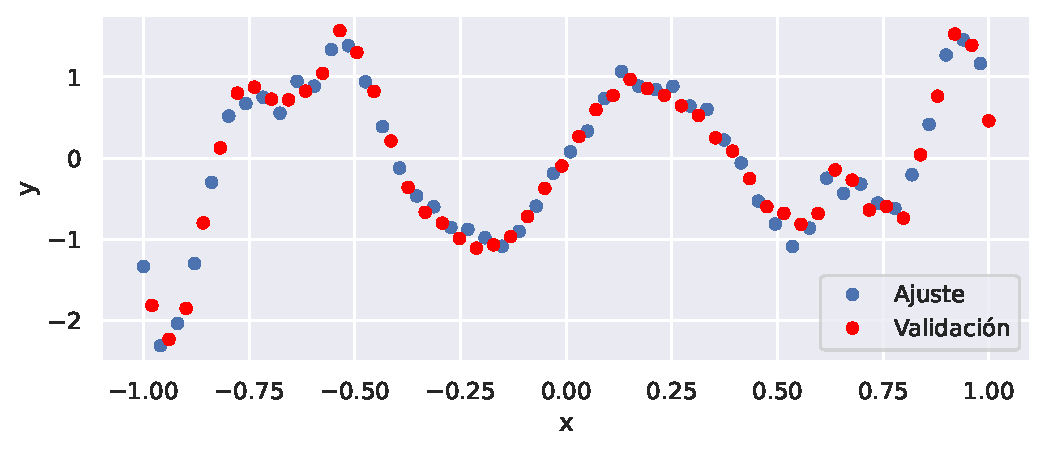
\includegraphics[width=0.85\textwidth]{img/scatterplot.pdf}
    \caption{
        Gráfico de dispersión del conjunto de datos. Se diferencian los datos pertenecientes a los conjuntos de ajuste y validación.
    } 
    \label{fig:scatterplot}
\end{figure}

El conjunto de datos que usamos está conformado por 100 observaciones de una variable $x$ y una variable $y$, particionados aleatoriamente en dos partes iguales, un conjunto de entrenamiento y un conjunto de validación (ver Figura \ref{fig:scatterplot}). A partir de estos datos, construimos la matriz $X$ según la expresión \ref{eq:matriz_x} con polinomios de Legendre de grado $d$.



Para hallar un modelo que generalice, buscamos el grado de polinomio $d$ y el valor de regularización $\lambda$ que minimizan el error de validación. En particular, tomamos como posibles valores $d={1, 2, \ldots, 49}$ y 100 valores $\lambda$ uniformemente distribuidos en una escala logarítimica en base 10 en el intervalo $[-7, 2]$, y evaluamos todas las combinaciones posibles (un total de $4900$ combinaciones). Para cada configuración, ajustamos el modelo con el algoritmo \ref{eq:cuadrados_svd_reg} en los datos de entrenamiento y evaluamos el ECM en los datos de validación según la expresión \ref{eq:ecm}.  

Realizamos todos los análisis y visualizaciones con Python 3.9. Para construir los polinomios de Legendre usamos la función \texttt{polynomial.legendre.legvander} de la biblioteca NumPy.



\section{Resultados} \label{sec:resultados}

En esta sección presentamos los resultados del análisis propuesto en la sección \ref{sec:experimentos}.

\begin{figure}[!ht]
    \centering
    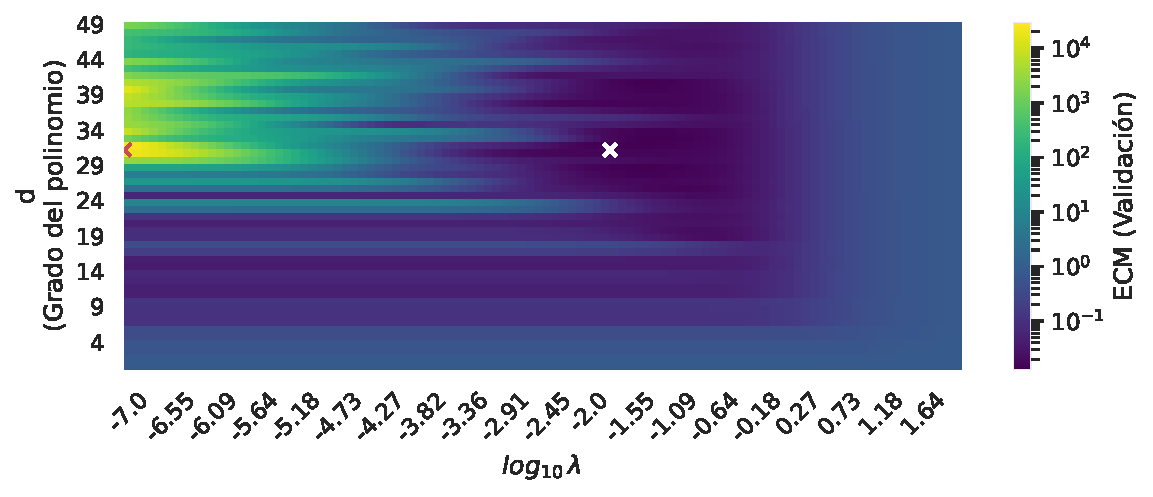
\includegraphics[width=0.85\textwidth]{img/heatmap.pdf}
    \caption{
        Mapa de calor que indica el error cuadrático medio de validación para la grilla de hiperparámetros explorada. En valores de $\lambda$ que exceden el rango visualizado, el error de validación no mejora. Se señala con una cruz blanca al punto asociado al par de ECM mínimo ($\lambda\approx 10^{-1.73}, d=32$), y con media cruz roja al asociado al de ECM máximo en todo el rango graficado ($\lambda=10^{-7}, d=32$).
    }
    \label{fig:heatmap}
\end{figure}

\clearpage
El ECM del ajuste a los datos de validación es mínimo para el polinomio de grado $d=32$ y coeficiente de regularización $\lambda \approx 10^{-1.73}$, con ECM $\approx 10^{-1.88}$. Casualmente, para el rango de hiperparámetros visualizado en el heatmap, $d=32$ es también el grado polinomial asociado al error máximo, con ECM $\approx 10^{4.47}$ (figura \ref{fig:heatmap}). El ajuste sobre los datos de validación mediante este polinomio puede ser visualizado en la figura \ref{fig:ajuste_mejor}.

\begin{figure}[!ht]
    \centering
    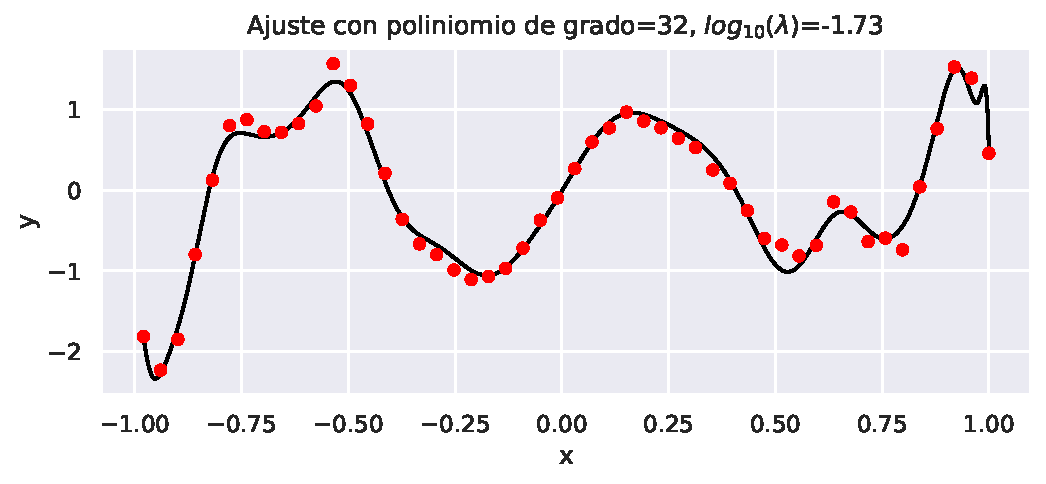
\includegraphics[width=0.85\textwidth]{img/ajuste_mejor.pdf}
    \caption{
        Valores ajustados del modelo con menor error de validación. En rojo, los datos de validación.
    } 
    \label{fig:ajuste_mejor}
\end{figure}

La figura \ref{fig:heatmap} expone varias propiedades interesantes del espacio de hiperparámetros ($\lambda$, $d$), que fueron exploradas en más profundidad en la figura \ref{fig:mas_ajustes} y que se comentan a continuación. 

Los máximos de ECM en todo el rango visualizado en el heatmap se encuentran en la región de alto grado polinomial y bajo coeficiente de regularización, donde es razonable que lo que esté ocurriendo sea un sobreajuste a los datos de entrenamiento y un consecuente mal ajuste en términos de ECM a los datos de validación. Esto puede visualizarse en la figura \ref{fig:ajuste_banda} para el caso particular con $d=32$, cuando se utilizan valores muy pequeños de $\lambda$. En relación a esto, una de las caracteristicas más llamativas del heatmap es la presencia de un bandeado horizontal para valores de $d$ suficientemente grandes ($d \gtrsim 20$), con la característica de que para $d$ fijo y al incrementar $\lambda$ el ECM tiende a primero disminuir hasta llegar a una región óptima para eventualmente volver a subir. Como puede visualizarse en la figura \ref{fig:ajuste_banda}, esto parece deberse a que con un primer incremento de $\lambda$ se logra disminuir el sobreajuste a los datos de entrenamiento; eventualmente se llega a un mínimo de ECM y el incremento de $\lambda$ más allá de este punto produce una disminución en la calidad del ajuste por exceso de regularización.

Para grados polinomiales muy bajos (alrededor de $d=3$) el ECM es, en terminos relativos a los errores en el resto del espacio, aproximadamente constante e independiente de $\lambda$ (moviendose horizontalmente a lo largo del heatmap con $d$ fijo). Esto evidentemente se debe a que cuando se tiene un grado polinomial demasiado bajo para los datos a ser ajustados, todo ajuste va a ser mediocre; no hay coeficiente de regularización que pueda salvar esa condición (figura \ref{fig:ajuste_grado_bajo}).

Finalmente, algo análogo ocurre para valores muy grandes de $\lambda$, más allá del valor óptimo hallado para $d=32$, para los cuales el ECM es aproximadamente constante e independiente del grado polinomial (moviendose verticalmente a lo largo del heatmap con $\lambda$ fijo). En este caso lo que ocurre es que para valores muy grandes de $\lambda$ el error de cuadrados mínimos pasa a ser dominado por el error de regularización, lo que produce que todos los coeficientes de la combinación lineal de polinomios de Legendre tiendan a 0, generandose como resultado un polinomio aproximadamente de la forma $f(x)=0$ independientemente del grado (figura \ref{fig:ajuste_exceso_ridge}).

\begin{figure}[htp]
\centering
    \subfloat[Polinomios de grado $d=32$ con coeficiente de regularización $\lambda$ variable. (*) Polinomio asociado al mejor ajuste (figuras \ref{fig:heatmap} y \ref{fig:ajuste_mejor}). En el gráfico de ECM en función de $\lambda$ se encuentra resaltado el punto asociado al polinomio. (**) Polinomio asociado al peor ajuste dentro del rango graficado en la figura \ref{fig:heatmap}.]{
    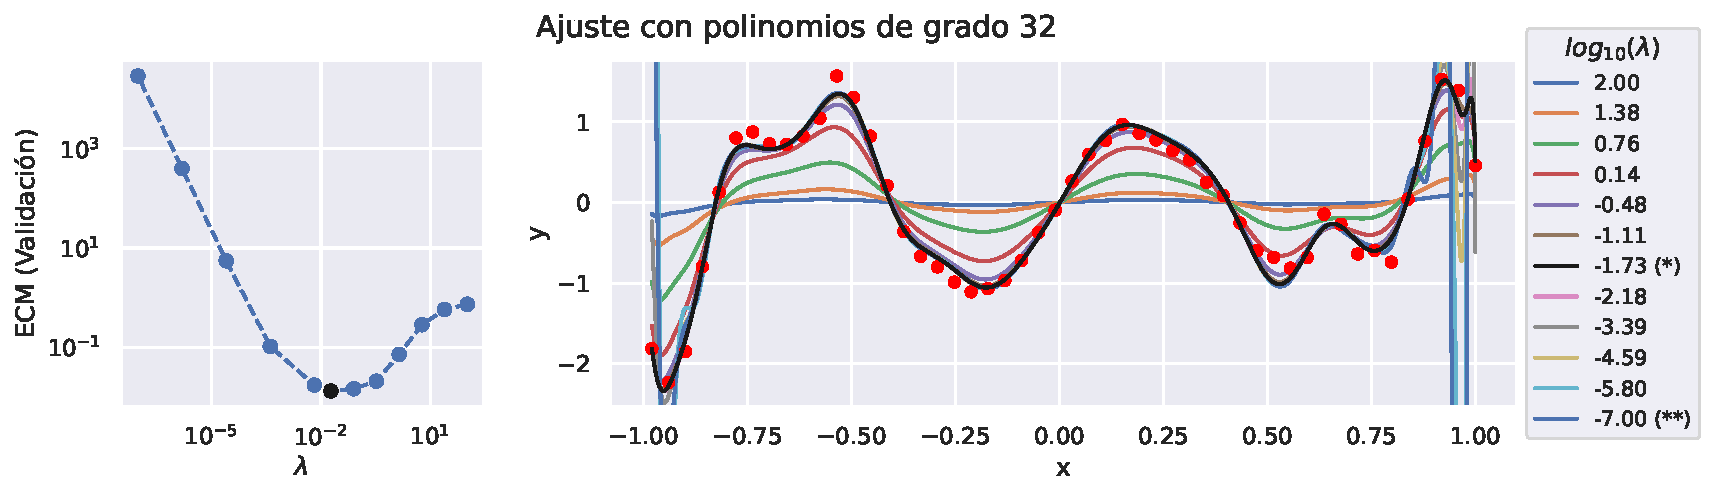
\includegraphics[width=1.0\textwidth]{img/ajuste_banda.pdf}
    \label{fig:ajuste_banda}
    }

    \subfloat[Polinomios de grado insuficiente $d=3$ con coeficiente de regularización $\lambda$ variable.]{
    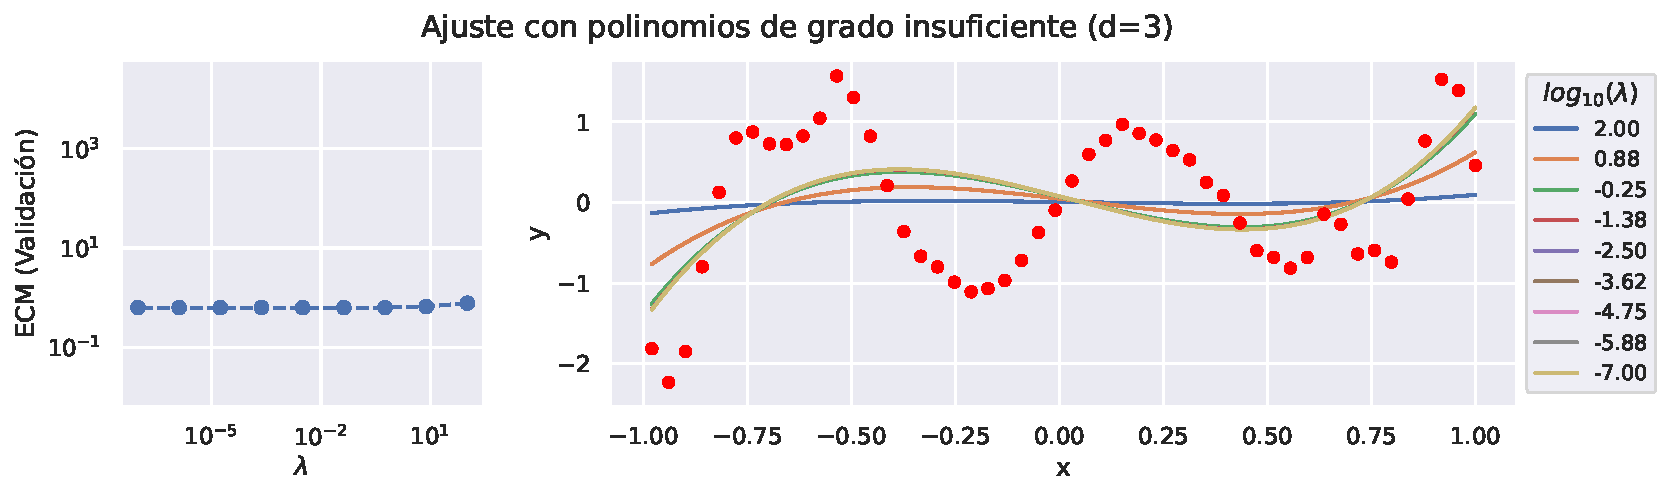
\includegraphics[width=1.00\textwidth]{img/ajuste_grado_bajo.pdf}
    \label{fig:ajuste_grado_bajo}
    }

    \subfloat[Polinomios de grado $d$ variable con coeficiente de regularización excesivo $\lambda=10$.]{
    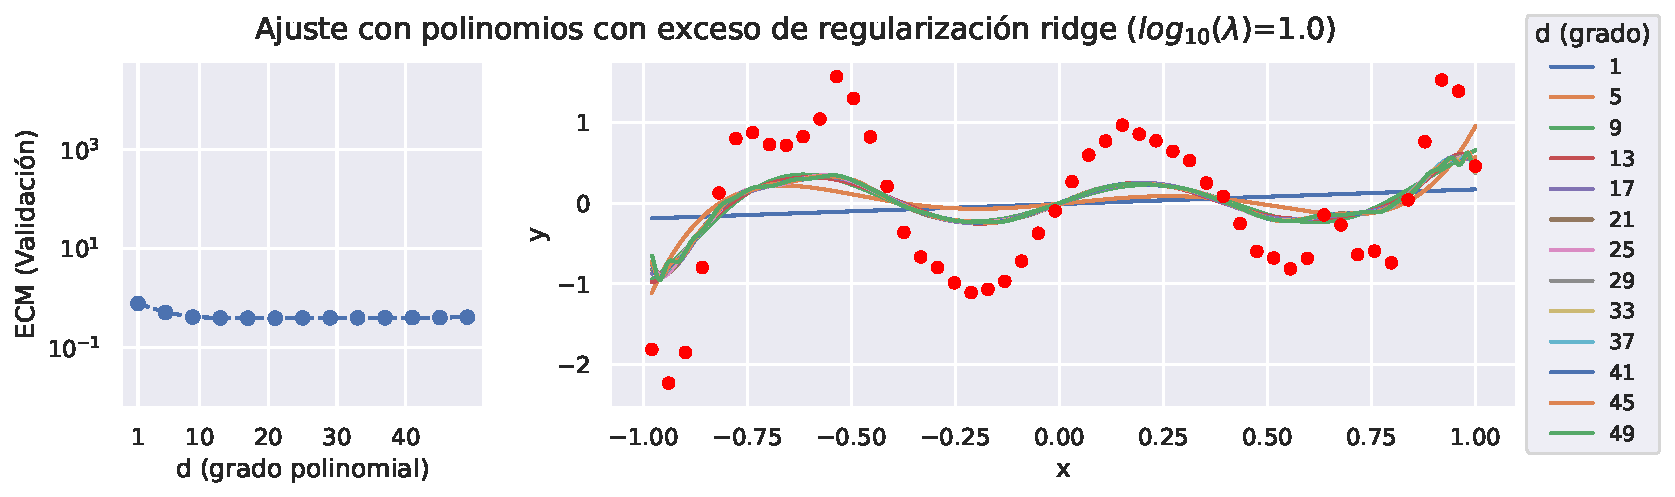
\includegraphics[width=1.0\textwidth]{img/ajuste_exceso_ridge.pdf}
    \label{fig:ajuste_exceso_ridge}
    }
    
    \caption{
        ECM y gráfico de ajuste a los datos de validación para polinomios asociados a series de pares ($\lambda, d$). En todos los casos se grafica a la izquierda el ECM de validación, en función de $\lambda$ en $(a)$ y $(b)$ y del grado polinomial en $(c)$, y a la derecha se muestran los ajustes correspondientes a cada valor del error, con los datos de validación en rojo. Para los gráficos de ECM se usó siempre la misma escala en el eje y con el fin facilitar la comparación de errores entre subfiguras.
    }
    \label{fig:mas_ajustes}
\end{figure}

\clearpage
\section{Conclusiones} \label{sec:conclusiones}

En este trabajo implementamos la solución al problema de mínimos cuadrados lineales mediante la descomposición SVD, con y sin regularización. También usamos la técnica de polinomios de Legendre para implementar regresión polinomial, la cual nos permite ajustar datos de manera no lineal resolviendo el problema de cuadrados mínimos lineales de manera computacionalmente eficiente. Mediante una aplicación práctica en la que buscamos el grado de polinomio y el valor de regularización que minimizan el error de validación, mostramos que la regularización es una estrategia efectiva para optimizar la capacidad predictiva de un modelo de ajuste.



%\section*{References}

%{
%\small

\bibliography{references}
\bibliographystyle{plainnat}

%}

%%%%%%%%%%%%%%%%%%%%%%%%%%%%%%%%%%%%%%%%%%%%%%%%%%%%%%%%%%%%

\end{document}

\clearpage
\section{Conclusiones}

Se diseñaron e implementaron algoritmos de EG para resolución de sistemas de ecuaciones lineales en Python, sin el uso de bibliotecas de álgebra lineal como Numpy o afines. Entre ellos, se diseñó un algoritmo de EG con pivoteo parcial (intercambio entre filas) que disminuye el error numérico, permite encontrar la solución de más sistemas, y no incrementa considerablemente la complejidad algoritmica respecto al algoritmo sin pivoteo, siendo ambos $O(n^3)$.

Aprovechando la estructura rala particular de las matrices tridiagonales, fue posible diseñar un algoritmo de EG de complejidad $O(n)$ que convierte a un sistema tridiagonal en uno equivalente diagonal a partir del cual es trivial encontrar la solución. Resolviendo sistemas tridiagonales dados por la matriz de la aproximación discreta al operador Laplaciano y varios vectores de términos independientes, se logró efectivamente encontrar aproximaciones discretas a funciones a partir de sus derivadas segundas.

Fue posible mejorar el algoritmo de EG para matrices tridiagonales de forma tal de permitir el precómputo de su sistema diagonal equivalente, permitiendo una disminución en tiempo de cómputo considerable para casos en los que es necesario reutilizar a una misma matriz de coeficientes para operar sobre una serie de vectores de términos independientes. Este último fue por ejemplo el caso de la simulación del proceso físico de difusión. Partiendo de la matriz tridiagonal asociada a la aproximación discreta a la ecuación de difusión, se precomputó su sistema diagonal equivalente y se lo resolvió iterativamente a partir de una condición inicial, efectivamente simulando la evolución temporal de la difusión a lo largo de un segmento lineal del espacio.

Para la cuantificación de los tiempos de cómputo de los distintos algoritmos se eligió una métrica robusta, el tiempo mínimo de los promedios de múltiples grupos de ejecuciones, mucho menos sensible al ruido propio del entorno en el que se ejecuta el código que otras como son el tiempo promedio. La medición de los tiempos nos permitió comprobar nuestros saberes previos acerca de cuales algoritmos esperabamos sean más rápidos, y con qué complejidades algorítmicas.

\clearpage
\begin{thebibliography}{999}
\label{sec:referencias}
\addcontentsline{toc}{section}{\nameref{sec:referencias}}

\bibitem{burden}
    Richard L. Burden, Douglas J. Faires \& Annette M. Burden,
    \emph{Numerical Analysis}, 10th ed.
    2016. \href{https://heavyphysicsblog.files.wordpress.com/2019/06/analisis-numerico-burden-faires-10ed.pdf}{\textbf{\textcolor{blue}{link}}}.

\bibitem{metnum_EG}
    Métodos Numéricos (UBA, FCEyN, DC),
    \emph{Sistemas de ecuaciones lineales y Eliminación Gaussiana}.
    Segundo cuatrimestre 2023. \href{https://heavyphysicsblog.files.wordpress.com/2019/06/analisis-numerico-burden-faires-10ed.pdf}{\textbf{\textcolor{blue}{link}}}.

\bibitem{timeit}
    Documentación oficial de \texttt{\%timeit}. \href{https://ipython.readthedocs.io/en/stable/interactive/magics.html#magic-timeit}{\textbf{\textcolor{blue}{link}}}.

\bibitem{patterson}
    David A. Patterson \& John L. Hennessy,
    \emph{Computer Organization and Design: The Hardware/Software Interface}, 3rd ed.
    2005. \href{https://ia600201.us.archive.org/24/items/ComputerOrganizationAndDesign3rdEdition/-computer%20organization%20and%20design%203rd%20edition.pdf}{\textbf{\textcolor{blue}{link}}}.

\end{thebibliography}

\clearpage
\section*{Apéndice}
% \label{sec:apendice}
\addcontentsline{toc}{section}{Apéndice}

Todo el código necesario para computar los resultados mostrados y discutidos en este informe puede encontrarse en y ser ejecutado desde la siguiente Jupyter notebook: \href{https://colab.research.google.com/drive/1AtO3fGa4pEk_aWhHOXmj6WMH6FihLcvY?usp=sharing}{\textbf{\textcolor{blue}{link}}}.

A continuación se comparten los pseudocódigos de algunos de los algoritmos auxiliares que fueron parte del diseño de los algoritmos principales ya presentados.

\begin{algorithm}[H]
\begin{algorithmic}[1]
\Require{$fila$, $columna$ vectores de dimensiones $1$\texttt{x}$n$ y $n$\texttt{x}$1$ respectivamente}
\Ensure{$res$ escalar tal que $fila \cdot columna=res$}
\Function{$producto\_escalar\_vector\_fila\_vector\_columna$}{$fila$, $columna$}
    \State $res \gets 0$
    \For{$i = 0 \hdots |fila|$}
        \State $res \gets res + fila[i]*columna[i]$
    \EndFor
    \State \textbf{return} $res$
\EndFunction
\end{algorithmic}
\caption{Producto escalar}
\label{alg:producto_escalar}
\end{algorithm}

\begin{algorithm}[H]
\begin{algorithmic}[1]
\Require{$A$, $B$ matrices de la misma dimensión}
\Ensure{$res$ matriz tal que $A+B=res$}
\Function{$suma\_matricial$}{$A$, $B$}
    \State $res \gets A$ \Comment{copia profunda}
    \For{$i = 0 \hdots |A|$}
        \For{$j = 0 \hdots |A[0]|$}
            \State $res[i][j] \gets A[i][j] + B[i][j]$
        \EndFor
    \EndFor
    \State \textbf{return} $res$
\EndFunction
\end{algorithmic}
\caption{Suma de matrices}
\label{alg:suma_matricial}
\end{algorithm}

\begin{algorithm}[H]
\begin{algorithmic}[1]
\Require{$A$ matriz}
\Require{$k$ escalar}
\Ensure{$res$ matriz tal que $kA=res$}
\Function{$producto\_por\_escalar$}{$A$, $k$}
    \State $res \gets A$ \Comment{copia profunda}
    \For{$i = 0 \hdots |A|$}
        \For{$j = 0 \hdots |A[0]|$}
            \State $res[i][j] \gets k*A[i][j]$
        \EndFor
    \EndFor
    \State \textbf{return} $res$
\EndFunction
\end{algorithmic}
\caption{Producto por escalar}
\label{alg:producto_por_escalar}
\end{algorithm}

\end{document}